%\subsubsection{SVT DAQ}



The SVT DAQ was a rapidly built DAQ  designed to readout data continuously at 40 MHz from the silicon detector modules, and transfer data to the JLab DAQ once a trigger signal is received. It is built using the same 
basic architecture and layout as the HPS DAQ but without the optical readout components and 
power distribution system inside the vacuum described in Sec.~\ref{sec:svt_daq}. 

The test run had a total of 20 silicon strip sensors, each one connected to an onboard hybrid readout card 
which is similar to the HPS hybrid, each one holding five 128-channel APV25 integrated circuits. The test 
run hybrid readout card is shown in Fig.~\ref{fig:hybrid_and_apv25_testrun} 
 \begin{figure*}[t]
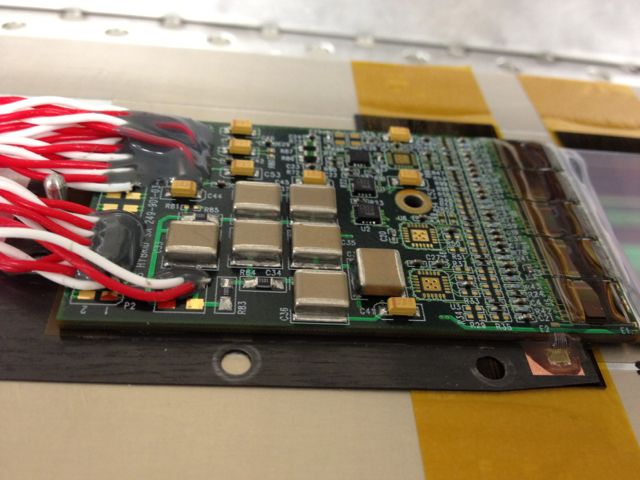
\includegraphics[ scale=0.3]{test2012/daq/hybrid.jpg}
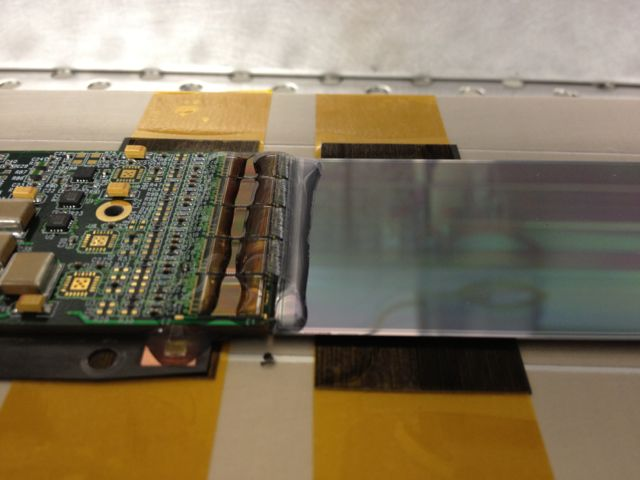
\includegraphics[ scale=0.3]{test2012/daq/apvs-on-hybrid.jpg}
\caption{\small{Picture of a test run hybrid readout board holding five APV25 ASICs. The wire bonds to the 
silicon sensors can be seen as well.}}
\label{fig:hybrid_and_apv25_testrun}
\end{figure*}

Contrary to the HPS DAQ where opto-boards digitize and converts the APV25 analog output signals to 
optical signals inside the vacuum chamber, the hybrids here carry analog signal directly to the 
Rear Transition Module (RTM) via a multi-twisted-pair cable. The amplification and digitization of the 
analog differential voltage output of the APV25 output are therefore carried out on the RTM board 
which was designed specifically for the HPS test run. Figure~\ref{fig:svtdaq} shows an overall layout of 
the SVT test run DAQ system (compare to Fig.~\ref{fig:svt_daq_overview}).
 \begin{figure}[t]
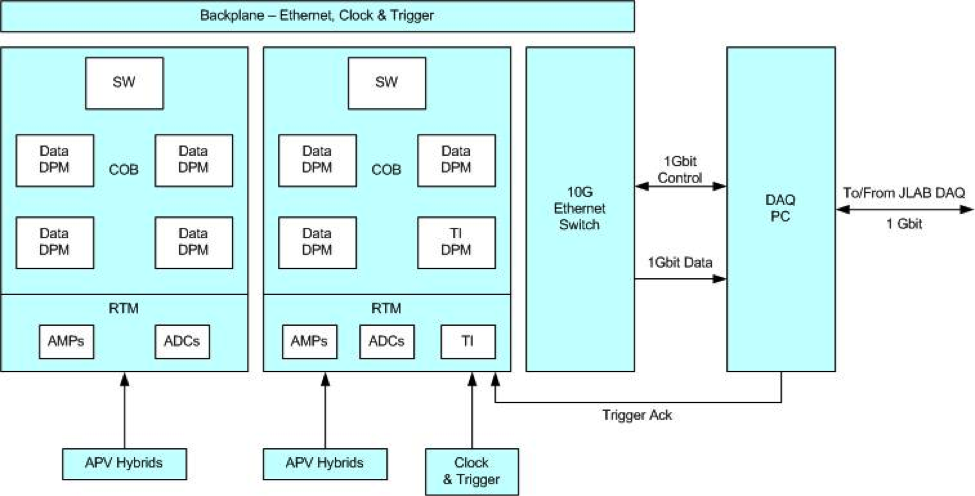
\includegraphics[scale=0.9]{test2012/daq/svt_daq_diagram.png}
\caption{\small{Schematic of the SVT DAQ showing input from the hybrids mounted on the silicon detector to the RTM, its connection to the COB, and the Ethernet switch used to transfer data at 1 Gbps to the 
DAQ PC and ultimately to the JLAB DAQ.}}
\label{fig:svtdaq}
\end{figure}
On the RTM, a pre-amplifier converts the APV25 differential current output to a different voltage output 
scaled to the sensitive range of a 14-bit ADC. The RTM is organized into four sections with each section 
supporting 3 hybrids (15 channels). 
The ADC is operated at the system clock of 41.667 Mhz. 
%The RTM also includes a 4-channel Fiber Optic module and supporting logic which can be used to interface to the JLAB trigger supervisor card.
The ATCA main board (the Cluster On Board or COB) is similar to the HPS DAQ with the important exception that one of the DPM's functions as the trigger interface only and there is no RCE module. 
Instead, the DPMs package and send the data from the hybrids to an external PC through a 1Gbps 
ethernet connection which serve the same purpose as the RCE module in the HPS DAQ. 
The ATCA crate hosts two COB cards, one supporting four data processing DPMs and the other supporting three data processing DPMs and one trigger DPM to support a total of 21 hybrids, one more than required. 
The test run RTM and COB can be seen in Fig.~\ref{fig:rtm_testrun}. 
\begin{figure*}[t]
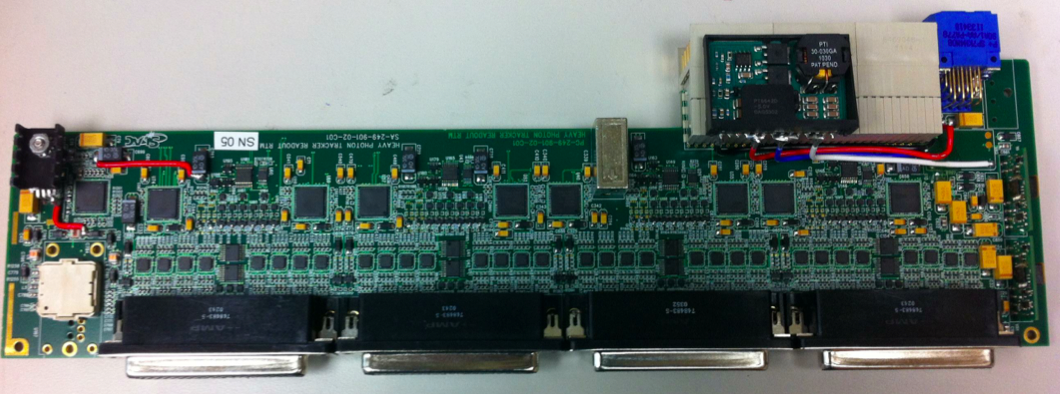
\includegraphics[ scale=0.25]{test2012/daq/rtm.png}
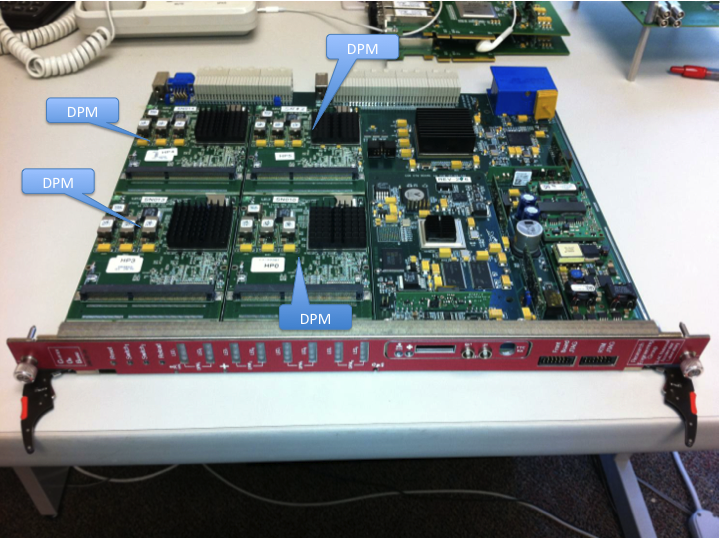
\includegraphics[ scale=0.4]{test2012/daq/svt_daq_module_noted.png}
\caption{\small{Picture of a RTM (top) and COB board (bottom) used in the HPS test run 2012.}}
\label{fig:rtm_testrun}
\end{figure*}
The external PC supports three network interfaces, 2 standard 1G-bit Ethernet and one custom low latency data reception card. The first Ethernet interface is used for slow control and monitoring of the 8 DPM modules. The second Ethernet interface serves as the interface to the JLAB data acquisition system. The third custom low latency network interface is used to receive data from the SVT ATCA crate and supports a low latency, reliable TTL trigger acknowledge interface to the trigger DPM. This PC hosts the SVT control and monitoring software as well as the JLAB ROC (Read Out Controller) application.
